\section{Prioritising Requirements}\label{section_riskVsValue}
\unsure{Tror det her afsnit skal laves om til mere project management}

Now that the object-oriented analysis and design has been concluded, and the functionalities has been laid out, it's time for the prioritising. Because of the limitations of the project some functionalities has to be downsized\todo{(removed from the scope?)}. This section will therefore explain the approach, as well as the prioritising based on both the problem statement but also the size of the project, with the use of the Value vs Complexity prioritization framework\ref{ValueVsComplexity}.

The Value vs Complexity framework works by having the individual members of the development team evaluate each functionality individually, and deciding on a value and a complexity.

\begin{itemize}
  \item \textbf{Value:} represented by a number between 0 and 100, where 100 means the functionality on its own will ???.
  
  \item \textbf{Complexity:} represented by a number between 0 and 100, where 100 means ???. \todo{Vælg standard}
\end{itemize}

In this project this task was performed without talking to each other nor showing what they decided upon. Afterwards, the team compared the results and the participants that differed the most from one another, would each explain why they evaluated it the way they did. After the explanation, the members of the group had the opportunity to change their evaluation. By using this approach, graph \ref{fig:ValueVsComplexity} was created. The data sheets for the graph can be found in appendix \ref{reqprio}.
%\todo{Ref til bilag til data skema. + fake data :kajez:}

\begin{figure}[H]
    \centering
	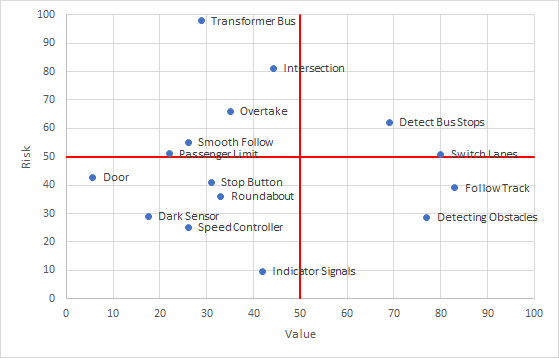
\includegraphics[width=0.9\textwidth]{Images/Graphs/RiskValue.png}
    \caption{Value Vs Complexity graph in a 2x2 grid.}
    \label{fig:ValueVsComplexity}
\end{figure}
\todo{Update billede}

As seen in figure \ref{fig:ValueVsComplexity} the plots have been sorted into a 2x2 grid, these four domains can be seen as the four criterias of the MoSCoW method: 
\begin{itemize}
    \item Must Have   (High value \& Low Complexity)
    \item Should Have (High Value \& High Complexity)
    \item Could Have  (Low Value \& Low Complexity)
    \item Won't Have  (Low Value \& High Complexity)
\end{itemize}

According to the framework, the development should start with the tasks in the "Must Have" domain, however this technique is no silver bullet, since it doesn't take into account relations and dependencies between functionalities independently of the model. Because of this \todo{Modifications Here if Any}.







% Now that the object-oriented analysis and design has been concluded, and the functionalities has been laid out, it's time for the prioritising. Because of the limitations of the project some functionalities has to be downsized(removed from the scope?). This section will therefor explain the approach, as well as the prioritising based on both the problem statement but also the size of the project, with the use of the Risk Vs Value model. 

% The Risk Vs Value model works by having the individual members of the development team evaluate each functionality individually, and giving them a risk and a value.
% \begin{itemize}
%   \item Value represented by a number between 0 and 100, where 100 means the functionality on its own will complete the project, and 0 provides nothing to the project.
  
%   \item Risks represented by a number between 0 and 100, where 100 means it will take the entire project to fulfil, and 0 is done without sacrificing any valuable time.
% \end{itemize}


% % http://www.project-management-knowhow.com/risk_management.html
% % MoSCoW method, måske brug det?
% % Value vs Complexity? http://www.product-arts.com/resourcemain/articlemenu/1049-value-vs-complexity-a-prioritization-framework




% In this project, all of the project members individually evaluated, importantly without talking to each other or knowing the evaluation of the other members beforehand. Afterwards, the team compared their results and the participants that differed the most from one another, would each explain why they evaluated it the way they did. After the explanation, the members of the group has the opportunity to change their evaluation. By using this approach, graph \ref{fig:RiskValueGraph} was created.
% \todo{Ref til bilag til data skema.}

% \begin{figure}[!ht]
%     \centering
% 	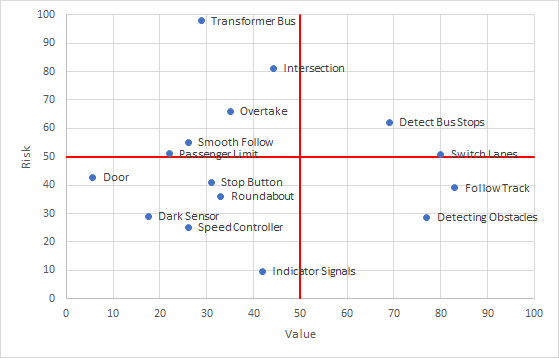
\includegraphics[width=0.9\textwidth]{Images/Graphs/RiskValue.png}
%     \caption{Risk Value Graph}
%     \label{fig:RiskValueGraph}
% \end{figure}

% According to the Risk Vs Value model, the development should start with the tasks with a high risk and value, proceeded by the tasks with low risk and high value, and lastly the tasks with a low value and low risk. Where the tasks with high risk and low value were of low priority, or completely ignored. 

% According to the graph, detecting bus stops is first priority\todo{Should it not be something else that is first priority, there are things with both higher value and lower risk.}, thereafter further functionality will be prioritised by iterating through the graph clockwise. Noteworthy is that the model is not bulletproof, and as such the relations and dependencies between the different functionality must be taken into account independently of the model.

% \subsection{Priority Modifications}

% In this section, we will give lower or higher priorities to some features, depending on the relations between the different features.

% All of the passenger functionality relies on the Bus being able to drive around first. Because of this, everything concerning passengers has been deemed of low priority. The same reason is used for overtakes. Detecting the darkness for turning on the lights is also given a low priority based on its low value.

% Following the track is crucial, and thus has been given the highest value, and as such has the highest priority.

% From this we determined the project requirements and they will be listed in the next section.
